
\documentclass[11pt]{article}
 
\usepackage[utf8]{inputenc}
\usepackage{hyperref}
\usepackage[margin=0.75in]{geometry} 
\usepackage{amsmath,amsthm,amssymb}

\usepackage{enumitem}
\usepackage{tcolorbox}
\usepackage{graphicx}
\usepackage{biblatex}
\addbibresource{ref.bib}

\usepackage{pythonhighlight}

\date{}
\begin{document}
 
% ////////////////////////////////////////////////////////////
%                         Info begins
% ////////////////////////////////////////////////////////////
 
\title{Resampling Methods for Algorithm Validation Applied to A Differently Transformed Data Set}
\author{Mariana Ávalos Arce \\Universidad Panamericana \\Data Mining, Fall 2021}

\maketitle

\begin{abstract}

The purpose of this document is to apply five resampling methods that are commonly used to validate Machine Learning Algorithms, in this case, Logistic Regression for a Classification problem. These resampling methods are: 1) Cross Validation, 2) Cross Validation with Repetitions, 3) Division by Percentage, 4) Division by Percentage Repeated and 5) Leave One Out Cross Validation; and these will be applied to three different versions of the same data set, which will be computed from the application of data transformations, leaving us with the three versions being Raw Data, Standardized Data and Standardized plus Yeo-Johnson Transformed Data. By applying the methods to the different versions of the data set, we will arrive at some important conclusions about what transformations seem to improve the quality of the data that will be the input for the ML algorithm, and also the differences in performance and execution of these Resampling Methods.
\end{abstract}

\begin{center}
\rule{0.7\textwidth}{.4pt}
\end{center}

\section{The Data Set}

The data set used in the following pages is owned by UCI Machine Learning \cite{bcancer:1}, and was found through Kaggle's data set browser. In simple words, this data set is used for a Supervised Classification Problem in which a Machine Learning algorithm learns to predict whether a female patient's breast tumor is malign or benign, given some attributes from said tumor. The features or attributes in the data set were extracted from digitized images of a breast cancer cell in different tumors, which describe the cell nuclei presented in the images. A brief description of each column or attribute is provided for clarity on further sections:
\\

\begin{tcolorbox}
\begin{enumerate}[nolistsep]
    \item \verb$id$: unique number of the patient.
    \item \verb$diagnosis$: M = malign or B = benign.
    \item \verb$radius_mean$: mean of distances from center to points on the perimeter.
    \item \verb$texture_mean$: standard deviation of gray-scale values found on the tumor's image.
    \item \verb$perimeter_mean$: mean size of the core tumor.
    \item \verb$area_mean$: mean area of the tumor.
    \item \verb$smoothness_mean$: mean of local variation in radius lengths that represent smoothness.
    \item \verb$compactness_mean$: mean of perimeter raised to the power of 2 over the area.
    \item \verb$concavity_mean$: mean of severity of concave portions of the tumor's contour.
    \item \verb$concave points$: mean for number of concave portions of the tumor's contour.
    \item \verb$symmetry_mean$: tumor's symmetry measure.
    \item \verb$fractal_dimension$: mean for "coastline approximation" - 1.
\end{enumerate}
\end{tcolorbox}

\section{Data Set Cleaning}

\subsection{Erasing Useless Columns}

For the purposes of training a Logistic Regression algorithm, we need to binarize the \verb$diagnosis$ column, so that instead of \verb$B$ and \verb$M$ we have \verb$0$ and \verb$1$ as the possible values for this attribute, making it our class column. Additionally, the \verb$id$ attribute does not represent a numeric column per se, because its values do not intervene in the classification of a tumor. Thus, this column will better be dropped, as well as a column named \verb$Unnamed: 32$ that unexpectedly appears at the end of all the mentioned columns, and is filled with \verb$NaN$ entries. In this way, we are making our data set to have \textbf{only numeric columns}, and \textbf{one binary class column} that determines the classification attribute, which makes our problem \textbf{supervised binary classification}. The following code snippet performs this data set operations.
\\

\begin{python}
import pandas as pd

url = 'db/data.csv'
bcancer = pd.read_csv(url, header=0)
bcancer['diagnosis'] = bcancer['diagnosis'].apply(lambda x: 1 if x == 'M' else 0)
del bcancer['Unnamed: 32']
del bcancer['id']
\end{python}

\subsection{Dropping Off Based On Correlation}

Now, after having our data set as only numeric columns, the next step is to look for \textbf{data redundancy}. An attribute (column or feature) of a data set is called \textbf{redundant} if it can be derived from any other attribute or set of attributes. This can be perfectly identified whenever a column presents a strong correlation to another attribute, which usually means a correlation close to 1. For a quick visualization of the correlations in the data set, a heat map is plotted using the calculated correlation with the \textit{Pearson} method for all the possible combinations of column pairs, presented in Figure \ref{fig:corr}.

\begin{figure}[!ht]
\centering
    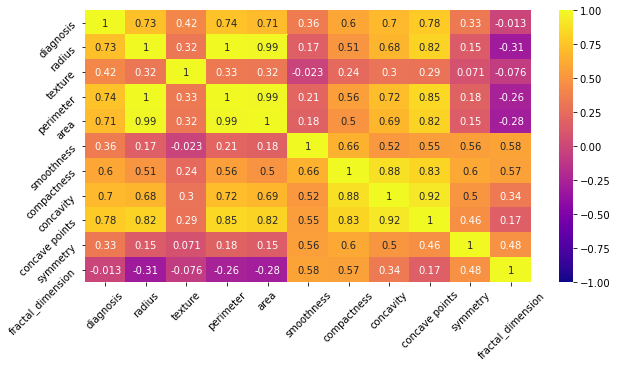
\includegraphics[width=5in]{correlation.png}
    \caption{Correlation heat map plot of all the data set attributes.}
    \label{fig:corr}
\end{figure}

Indeed there are some strongly correlated attributes, which show values close to 1, such as: \verb$perimeter$, \verb$area$ and \verb$radius$. The attributes \verb$perimeter$ and \verb$area$ present a correlation of 0.99 because of their calculation involving other similar measures, but they are completely different measures of the main properties of the tumor, so they were not dropped from the data set. Thus, the only pair remaining with a strong correlation value is \verb$radius$ and \verb$perimeter$. Which one to delete? The column \verb$perimeter$ presents a correlation of 0.74 with the \verb$diagnosis$ class column, whereas the column \verb$radius$ presents a correlation of 0.73 with the \verb$diagnosis$, therefore, \verb$radius$ can be considered as redundant, and thus is dropped from the data set. In other words, we delete the radius attribute due to its redundancy and lower relationship with the class. This operation is shown in the snippet below.
\\

\begin{python}
del df['radius_mean']
df.head()
\end{python}

At the end of these operations we can observe some instances that are left in the data set, shown in Table \ref{tab:head}.

\begin{center}
\begin{table}
\footnotesize
\begin{tabular}{ |c|c|c|c|c|c|c|c|c|c| } 

\hline
class & texture & perimeter & area & smoothness & compactness & concavity & concave points & symmetry & fractal\\
\hline
1 & 10.38 & 122.80 & 1001.0 & 0.1184 & 0.2776 & 0.3001 & 0.1471 & 0.2419 & 0.07871 \\ 
1 & 17.77 & 132.90 & 1326.0 & 0.08474 & 0.07864 & 0.0869 & 0.07017 & 0.1812 & 0.05667 \\
1 & 21.25 & 130.00 & 1203.0 & 0.10960 & 0.15990 & 0.1974 & 0.12790 & 0.2069 & 0.05999 \\
1 & 20.38 & 77.58 & 386.1 & 0.14250 & 0.28390 & 0.2414 & 0.10520 & 0.2597 & 0.09744 \\
1 & 14.34 & 135.10 & 1297.0 & 0.10030 & 0.13280 & 0.1980 & 0.10430 & 0.1809 & 0.05883 \\
\hline

\end{tabular}
\caption{\label{tab:head}Instances after cleaning operations (diagnosis is class).}
\end{table}
\end{center}

Thus, our data set seems ready to be plugged into the learning models. It is also important to mention that after performing the following,
\\

\begin{python}
benign = df.groupby('diagnosis').size()[0]
malign = df.groupby('diagnosis').size()[1]
total = malign + benign
benign_p = benign / (total) * 100
malign_p = malign / (total) * 100
print(f"benign: {benign_p:.2f}%")
print(f"malign: {malign_p:.2f}%")
\end{python}

we can see that 62.74\% of the instances correspond to class 0 and 37.26\% belongs to class 1. These percentages, although different, can say the data set is somehow balanced in terms of number of instances per class, to avoid an over-training of the model towards a specific class value, which would arise if the percentages differed much more.

\section{Resampling Methods: Cross Validation }

\subsection{Raw Data}

The first Resampling Method is the Cross Validation, in which we split the data into N parts and dedicate 1 to test the model and the N-1 remaining to train it, and iterate N times, each time changing the test part. We apply this method to \textbf{raw data}, which means that the \textbf{x} varibale containg a matrix of the data set values \textbf{without any transformation}, and the class column left out. The Logistic Regression needed in this case around \textbf{3500 iterations}. The \textbf{y} variable refers to our class column.
\\

\begin{python}
num_folds = 10
kfold = KFold(n_splits=num_folds, shuffle=True) 
model = LogisticRegression(solver='lbfgs', max_iter=3500)
results = cross_val_score(model, x, y, cv=kfold)
acc = results.mean() * 100 
stdev = results.std()
print(f"accuracy: {acc:.2f}% std: {stdev:.2f}")
\end{python}

As a result we get an \textbf{accuracy of 90.51\% and a standard deviation of 0.0335} for this method applied with raw data. Requiring 3500 iterations for the ML modeling seems risky, since this is a method that can potentially involve repetitions, and thus cost a lot more time, computationally speaking. With further methods this will show up more clearly.

\subsection{Standardized Data}

Now we will transform the \textbf{x} data matrix using a transformation called Standardization. This operation on \textbf{x} involves that, for each column $x_i$, the following is applied to get every instance:

\begin{equation}
    x_{scaled}=\frac{x_i-min(x_i)}{max(x_i)-min(x_i)}
\end{equation}

This transformation moves the attribute distribution towards a mean of zero and a standard deviation of 1. If we plot the new standardized data columns, we can see such results as in Figure \ref{fig:stand}. This transformation only translates the distribution to a more centered range, in simple words; this means that the distribution of the attributes is not modified towards a complete Gaussian bell, because its purpose is to standardize the ranges of values. This standardized data set will be called now \textbf{rescaled x}.
 
\begin{figure}[!ht]
\centering
    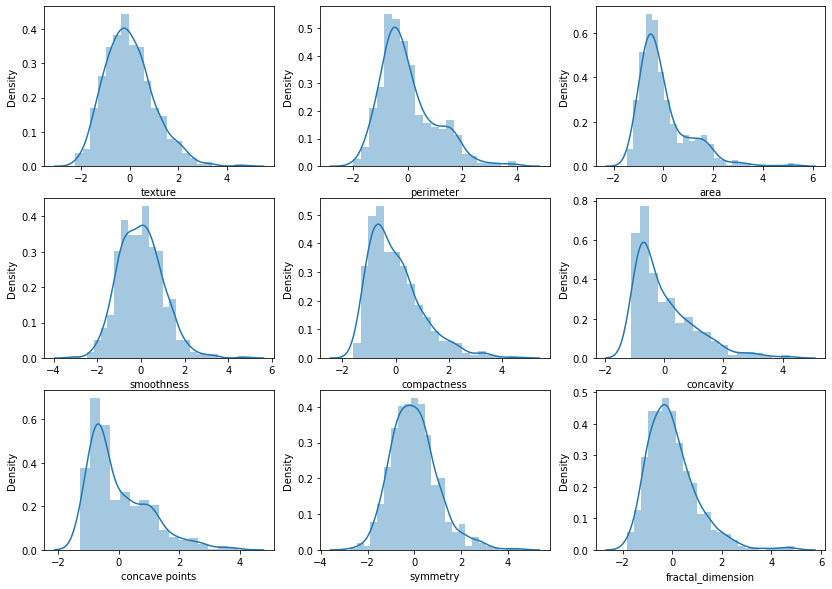
\includegraphics[width=6in]{rescaledX.png}
    \caption{Rescaled x: Standardized data attributes.}
    \label{fig:stand}
\end{figure}

\begin{python}
num_folds = 10
kfold = KFold(n_splits=num_folds, shuffle=True) 
model = LogisticRegression(solver='lbfgs', max_iter=100)
results = cross_val_score(model, rescaledX, y, cv=kfold)
acc = results.mean() * 100
stdev = results.std()
print(f"accuracy: {acc:.2f}% std: {stdev:.2f}")
\end{python}

The code snippet above outputs an \textbf{accuracy of 94.19\% and a standard deviation of 0.024} for the method applied to standardized data. Compared to the method in raw data, the accuracy in the prediction of the class by the model increased significantly from 90.51\% to 94.19\%, but more importantly, the iterations needed were reduced so that the model can converge in just 100 iterations, \textbf{reducing the computation time and increasing the accuracy}. 

\subsection{Standardization and Yeo-Johnson Transformed Data}

The \textbf{rescaled x} matrix of instances, as seen in Figure \ref{fig:stand}, is centered in a mean of zero and has a unit standard deviation, but it can suffer further transformations so that the column instances have a more Gaussian-like distribution. This transformation can be achieved by using either the \textit{Box-cox method} or the \textit{Yeo-Johnson method}, but in this case the \textit{Yeo-Johnson method} is the only one of the two that accepts negative data values, such as the ones present in our data set. The method tries to fit the best parameters to achieve a Gaussian bell with each of the \textbf{rescaled x} attributes, producing an x matrix we will refer as \textbf{transformed x}, plotted in Figure \ref{fig:yeo}.
\\

\begin{figure}[!ht]
\centering
    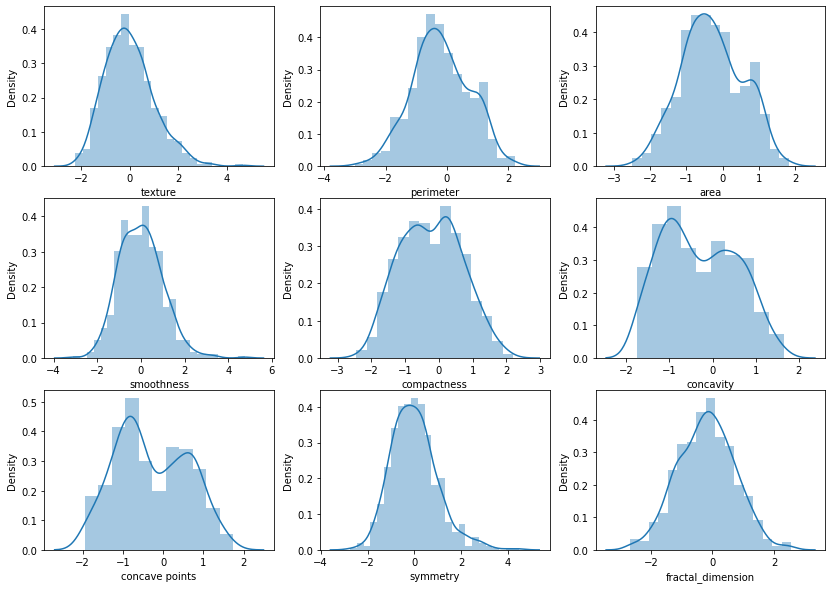
\includegraphics[width=6in]{transformedX.png}
    \caption{Transformed x: Standardized and Yeo-Johnson transformed data attributes.}
    \label{fig:yeo}
\end{figure}

If we compare Figure \ref{fig:stand} and Figure \ref{fig:yeo}, we can see that not every column was transformed by Yeo-Johnson's method, because not all attributes seemed to have a significant enough skewness to be transformed, such is the case of \verb$texture$,  \verb$smoothness$ and  \verb$symmetry$ columns. This was conlcuded after analysing which box plots presented a strong skewness towards some side of the other, such the top plot in Figure \ref{fig:boxplots}. As a result, the bottom plot in Figure \ref{fig:boxplots} shows also how the \textbf{number of atypical instances was reduced by Yeo-Johnson's method}, which most of the times reduces the solution search process in a Machine Learning algorithm.
\\

\begin{figure}[!ht]
\centering
    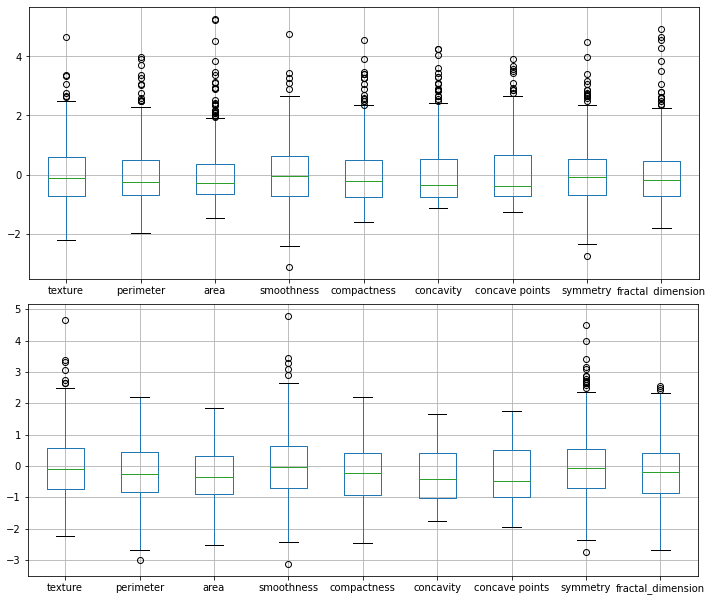
\includegraphics[width=5.5in]{box-plots.png}
    \caption{Rescaled x (top) Transformed x (bottom): box plots.}
    \label{fig:boxplots}
\end{figure}

With \textbf{transformed x} matrix ready, we compute now the Cross Validation to this data in the code snippet below.
\\

\begin{python}
num_folds = 10
kfold = KFold(n_splits=num_folds, shuffle=True) 
model = LogisticRegression(solver='lbfgs', max_iter=100)
results = cross_val_score(model, transformedX, y, cv=kfold)
acc = results.mean() * 100 # percentage of accuracy
stdev = results.std() * 100
print(f"accuracy: {acc:.2f}% std: {stdev:.2f}%")
\end{python}

Unfortunately, the \textbf{accuracy did not increase from last method, since now we get 91.56\% with a stdev of 0.0271}, but it does increase with respect to the method applied in raw data. The algorithm also converges in around 100 iterations, so this method also involves a reduction from computation time when compared to raw data.

\section{Resampling Methods: Cross Validation with Repetitions}

\subsection{Raw Data}

Next up, the Cross Validation with Repetitions consists in, as its name implies, the performance of repeated Cross Validation methods. But, why would it help to repeat this method over and over? Because Cross Validation itself chooses the part that will be test \textbf{randomly}, and thus, by repeating it several times, we will reach further testing of our data with different combinations of N sets. We go back to applying this method to the raw data matrix \textbf{x}, as in the code snippet below.
\\

\begin{python}
num_folds = 10
num_repeated = 5
repeatedkfold = RepeatedKFold(n_splits=num_folds, n_repeats=num_repeated)
model = LogisticRegression(solver='lbfgs', max_iter=3500)
results = cross_val_score(model, x, y, cv=repeatedkfold)
acc = results.mean() * 100 # percentage of accuracy
stdev = results.std()
print(f"accuracy: {acc:.2f}% std: {stdev:.2f}")
\end{python}

Did it help? Well, the \textbf{accuracy in prediction was raised from 90.51\% to 90.65\% and the standard deviation from 0.0335 to 0.0370 with respect to Cross Validation with raw data}, which is somehow a growth in accuracy when raw data is used, but it is so small that it is likely to be insignificant and variate because of the randomness of the method. The fact that the standard deviation grew also a small bit is probably due to the fact that we simply have now more combinations of sets. Thus, at least with this data set, the repeated Cross Validation seems to be redundant and not significantly helpful when it comes to using raw data.

\subsection{Standardized Data}

Taking back the \textbf{rescaled x} data matrix, which is plotted in Figure \ref{fig:stand}, now it is time to see if the small increase in accuracy with raw data becomes a more significant increase in accuracy when applied to the standardized \textbf{x} matrix. We perform this Cross Validation with Repetitions below.
\\

\begin{python}
num_folds = 10
num_repeated = 5
repeatedkfold = RepeatedKFold(n_splits=num_folds, n_repeats=num_repeated)
model = LogisticRegression(solver='lbfgs', max_iter=100)
results = cross_val_score(model, rescaledX, y, cv=repeatedkfold)
acc = results.mean() * 100
stdev = results.std()
print(f"accuracy: {acc:.2f}% std: {stdev:.2f}")
\end{python}

The actual result was \textbf{the decrease to 93.85\% prediction accuracy and 0.0326 standard deviation decrease as well}, and this decrease may mean the model without the repetitions was a bit over-trained and now with more sets of testing and training, we reduced this 94\% accuracy to a 93\% due to the bigger amount of combinations.

\subsection{Standardization and Yeo-Johnson Transformed Data}

Now that we know what and why use Yeo-Johnson method, we can go back to the \textbf{transformed x} matrix, which includes standardization and Yeo-Johnson transform the the raw \textbf{x}.
\\

\begin{python}
num_folds = 10
num_repeated = 5
repeatedkfold = RepeatedKFold(n_splits=num_folds, n_repeats=num_repeated)
model = LogisticRegression(solver='lbfgs', max_iter=100)
results = cross_val_score(model, transformedX, y, cv=repeatedkfold)
acc = results.mean() * 100
stdev = results.std()
print(f"accuracy: {acc:.2f}% std: {stdev:.2f}")
\end{python}

Interestingly, the same thing occurred when we compared the Cross Validation with raw data to Cross Validation with Standard and Yeo's method, \textbf{we go from 90\% to 91.60\% accuracy}, while the highest (93.85\%) accuracy was reached with only the Standard Transformation. The fact that the same behaviour from the simple Cross Validation and Cross Validation with Repetitions happens tells us that maybe \textbf{the iterative process in still redundant and gives the same results with or without the repetitions}.

\section{Resampling Methods: Division by Percentage}

\subsection{Raw Data}

Now we will validate our Logistic Regression model with another technique called Division by Percentage, which consists in splitting the data set \textbf{x} into two parts only, but how big are these parts? The two parts will be divided following a given percentage, often 33\% for the training and the remaining 67\% for the testing or validation. This splitting is also random, but done once.
\\

Let's use the raw data matrix \textbf{x} and apply this method to the trained model. Such code snippet is below.
\\

\begin{python}
test_size = 0.33
seed = 1
x_train, x_test, y_train, y_test = train_test_split(x, y, test_size = test_size, random_state = seed)
model = LogisticRegression(solver='lbfgs', max_iter=3500)
model.fit(x_train, y_train)
results = model.score(x_test, y_test)
acc = results * 100
print(f"accuracy: {acc:.2f}%")
\end{python}

The output in this case was \textbf{87.3\% of prediction accuracy}, which is quite lower compared to the two methods seen before, with or without raw data. This is probably due to the method itself: it is just splitting and testing \textbf{once}, whereas the previous two methods involve inner iterations in the method itself. This method \textbf{lowers the accuracy level but also decreases the computation time and complexity}.

\subsection{Standardized Data}

Let us locate ourselves again with the standardized x matrix, called \textbf{rescaled x} and plotted in Figure \ref{fig:stand}, and try to apply this method to see how the model is validated: let's see the accuracy with \textbf{rescaled x}.
\\

\begin{python}
test_size = 0.33
seed = 1
x_train, x_test, y_train, y_test = train_test_split(rescaledX, y, test_size = test_size, random_state = seed)
model = LogisticRegression(solver='lbfgs', max_iter=100)
model.fit(x_train, y_train)
results = model.score(x_test, y_test)
acc = results * 100
print(f"accuracy: {acc:.2f}%")
\end{python}

The results here are very worth noticing. Compared to the method with raw data, this method with standardized data \textbf{increases the prediction accuracy from 87.3\% to 93.1\%, which is the biggest percentage increase so far}. With a reduced computation time such as the one needed for a Division by Percentage Validation, we can achieve similar accuracy results to the ones by Cross Validation and Cross Validation Repeated, which may be a crucial conclusion if our model needs large amounts of data and the computation time is an important issue.

\subsection{Standardization and Yeo-Johnson Transformed Data}

Changing our data back to \textbf{transformed x}, which is transformed by Standardization and Yeo-Johnson's Method, let's take a look at what the validation accuracy is with the code snippet below.
\\

\begin{python}
x_train, x_test, y_train, y_test = train_test_split(transformedX, y, test_size = test_size, random_state = seed)
model = LogisticRegression(solver='lbfgs', max_iter=100)
model.fit(x_train, y_train)
results = model.score(x_test, y_test)
acc = results * 100
print(f"accuracy: {acc:.2f}%")
\end{python}

Once again, we see that by taking \textbf{transformed x} as the input data, \textbf{the prediction accuracy increases (91.49\%), but not as much as with the standardized data}. This seems to be quite interesting, since the Yeo-Johnson transforms the set to be more similar to a Gauss bell, which is the data that a Machine Learning model such as Logistic Regression expects and works best with. This certainly will be addressed in the final conclusions of this document, as it seems to happen in all methods.

\section{Resampling Methods: Division by Percentage with Repetitions}

\subsection{Raw Data}

As mentioned above, the Division by Percentage method operates only one split and test over the input data, but takes the 33\% randomly. Now, taking advantage of that randomness, there exists another variation of this method called Division by Percentage with Repetitions. This method validates our model by taking 33\% for testing and 67\% of our data as training, but several times, since the split is done randomly. This method looks similar to what a simple Cross Validation does, because it makes N iterations to shuffle the part taken as test around our data set. The code snippet below shows the implementation of a Division by Percentage with Repetitions method with raw data matrix \textbf{x}.

\begin{python}
test_size = 0.33
n_splits = 10
kfold = ShuffleSplit(n_splits=n_splits, test_size = test_size)
model = LogisticRegression(solver='lbfgs', max_iter=3500)
results = cross_val_score(model, x, y, cv=kfold)
acc = results.mean() * 100
stdev = results.std()
print(f"accuracy: {acc:.2f}% std: {stdev:.2f}")
\end{python}

With raw data, we get \textbf{a prediction accuracy of 91.38\% and a std deviation of 0.016}, which means that if we perform the same method of Division by Percentage over and over (10 times in this case), the accuracy of the model with respect to the correct and known \textbf{y} increases from \textbf{87\% to around 91\%} using raw data, which is the same 91\% we get from Division by Percentage with \textbf{transformed x}, but by doing so simply with raw data \textbf{x}. Thus, we can say that Division by Percentage with Repetitions applied to raw data has the same output as a Simple Division by Percentage done with Standardized and Yeo-Johnson transformations.

\subsection{Standardized Data}

Taking back the Standradized matrix \textbf{rescaled x}, we can apply the Repeated Division by Percentage:
\\

\begin{python}
test_size = 0.33
n_splits = 10
kfold = ShuffleSplit(n_splits=n_splits, test_size = test_size)
model = LogisticRegression(solver='lbfgs', max_iter=100)
results = cross_val_score(model, rescaledX, y, cv=kfold)
acc = results.mean() * 100
stdev = results.std()
print(f"accuracy: {acc:.2f}% std: {stdev:.2f}")
\end{python}

Similarly, using the standard matrix we get \textbf{93.67\% of prediction accuracy and a standard deviation of 0.0094}, which is the smallest deviation we have got in any previous method, showing that the accuracy results in each repetition do not vary a lot throughout the 10 iterations. This can mean that the repetitions may be unnecessary, which is somehow shown also in the accuracy itself, because from raw data and standardized data we only increased around 2\%, whereas other methods applied to standard data show a bigger increase.

\subsection{Standardization and Yeo-Johnson Transformed Data}

We can apply this method of validation now with \textbf{transformed x}, which includes Standard and Yeo-Johnson transfoms, to see if redundancy is also suggested:
\\

\begin{python}
test_size = 0.33
n_splits = 10
kfold = ShuffleSplit(n_splits=n_splits, test_size = test_size)
model = LogisticRegression(solver='lbfgs', max_iter=100)
results = cross_val_score(model, transformedX, y, cv=kfold)
acc = results.mean() * 100
stdev = results.std()
print(f"accuracy: {acc:.2f}% std: {stdev:.2f}")
\end{python}

Interestingly, we got \textbf{accuracy of 91.97\% and standard deviation of 0.0018}, which is almost the same accuracy result we got with this same method but with raw data, but slightly bigger this time. This is a strange behaviour, since we were noticing that with \textbf{transformed x} the accuracy in prediction grew a bit more than just 0.59\%. This might show that this method done over and over is not really being helped in accuracy by the transformations, but these just reduce the computing time from 3500 iteration to 100 iterations in the model convergence itself.

\section{Resampling Methods: Leave One Out Cross Validation}

\subsection{Raw Data}

Finally we have reached the last validation method in the scope of this document: Leave One Out Cross Validation. What this means is, in iteration 1, what it does is take just one column as test data and the remaining columns as training data, and so on. Depending on the number of columns (N), the number of iterations there will be. We basically take all data values as training except one, instead of a percentage, which goes to test. The standard deviation will be higher, because we will be comparing one data value against its predicted value for an error estimation. Let's see how this performs with raw data \textbf{x}:
\\

\begin{python}
loocv = LeaveOneOut()
model = LogisticRegression(solver='lbfgs', max_iter=3500)
results = cross_val_score(model, x, y, cv=loocv)
acc = results.mean() * 100
stdev = results.std()
print(f"accuracy: {acc:.2f}% std: {stdev:.2f}")
\end{python}

Surprisingly, this method took over 12 seconds to output the result, which is quite noticeable compared to all the other methods that take at best 1 second to output the calculations. Either way, we get \textbf{accuracy in prediction of 90.69\% and a standard deviation of 0.29} which is similar to Cross Validation, Cross Validation Repeated and Division by Percentage Repeated, but done in much more time, whic might look as a disadvantage of this method, but quite logical due to the amount of iterations depending on the data set columns.

\subsection{Standardized Data}

Taking back the Standradized matrix \textbf{rescaled x} in Figure \ref{fig:stand}, we can apply the Leave One Out CV:
\\

\begin{python}
loocv = LeaveOneOut()
model = LogisticRegression(solver='lbfgs', max_iter=100)
results = cross_val_score(model, rescaledX, y, cv=loocv)
acc = results.mean() * 100
stdev = results.std()
print(f"accuracy: {acc:.2f}% std: {stdev:.2f}")
\end{python}

Not surprisingly, the \textbf{accuracy increased 94.20\% and the standard deviation decreased to 0.23}, which is quite the same increase from raw to standard data we have seen in all the previous methods. But now, the computation time is not so large as this time it took around 2 seconds, which confirms in a more exaggerated way that \textbf{the standardization of data reduces computation time since it makes the Logistic Regression converge faster in less iterations}.

\subsection{Standardization and Yeo-Johnson Transformed Data}

Changing our data back to \textbf{transformed x}, which is transformed by Standardization and Yeo-Johnson's Method, let's take a look at what the validation accuracy is with the code snippet below and the Leave One out CV method.
\\

\begin{python}
loocv = LeaveOneOut()
model = LogisticRegression(solver='lbfgs', max_iter=100)
results = cross_val_score(model, transformedX, y, cv=loocv)
acc = results.mean() * 100
stdev = results.std()
print(f"accuracy: {acc:.2f}% std: {stdev:.2f}")
\end{python}

This result was almost exactly the same as the one with raw data \textbf{x}, where now the \textbf{accuracy is  91.74\% with a standard deviation of 0.27}, but slightly increased and done also in 100 iterations (2 seconds), compared to the 3500 iterations that raw data required. Thus, the process done using \textbf{rescaled x} shows a bigger accuracy percentage, which has been happening with all methods.

\section{Overall Conclusions}

All the accuracy percentages we discussed might look at this point confusing and hard to synthesize, that is why all the accuracy throughout the different methods are plotted in Figure \ref{fig:bars}.

\begin{figure}[!ht]
\centering
    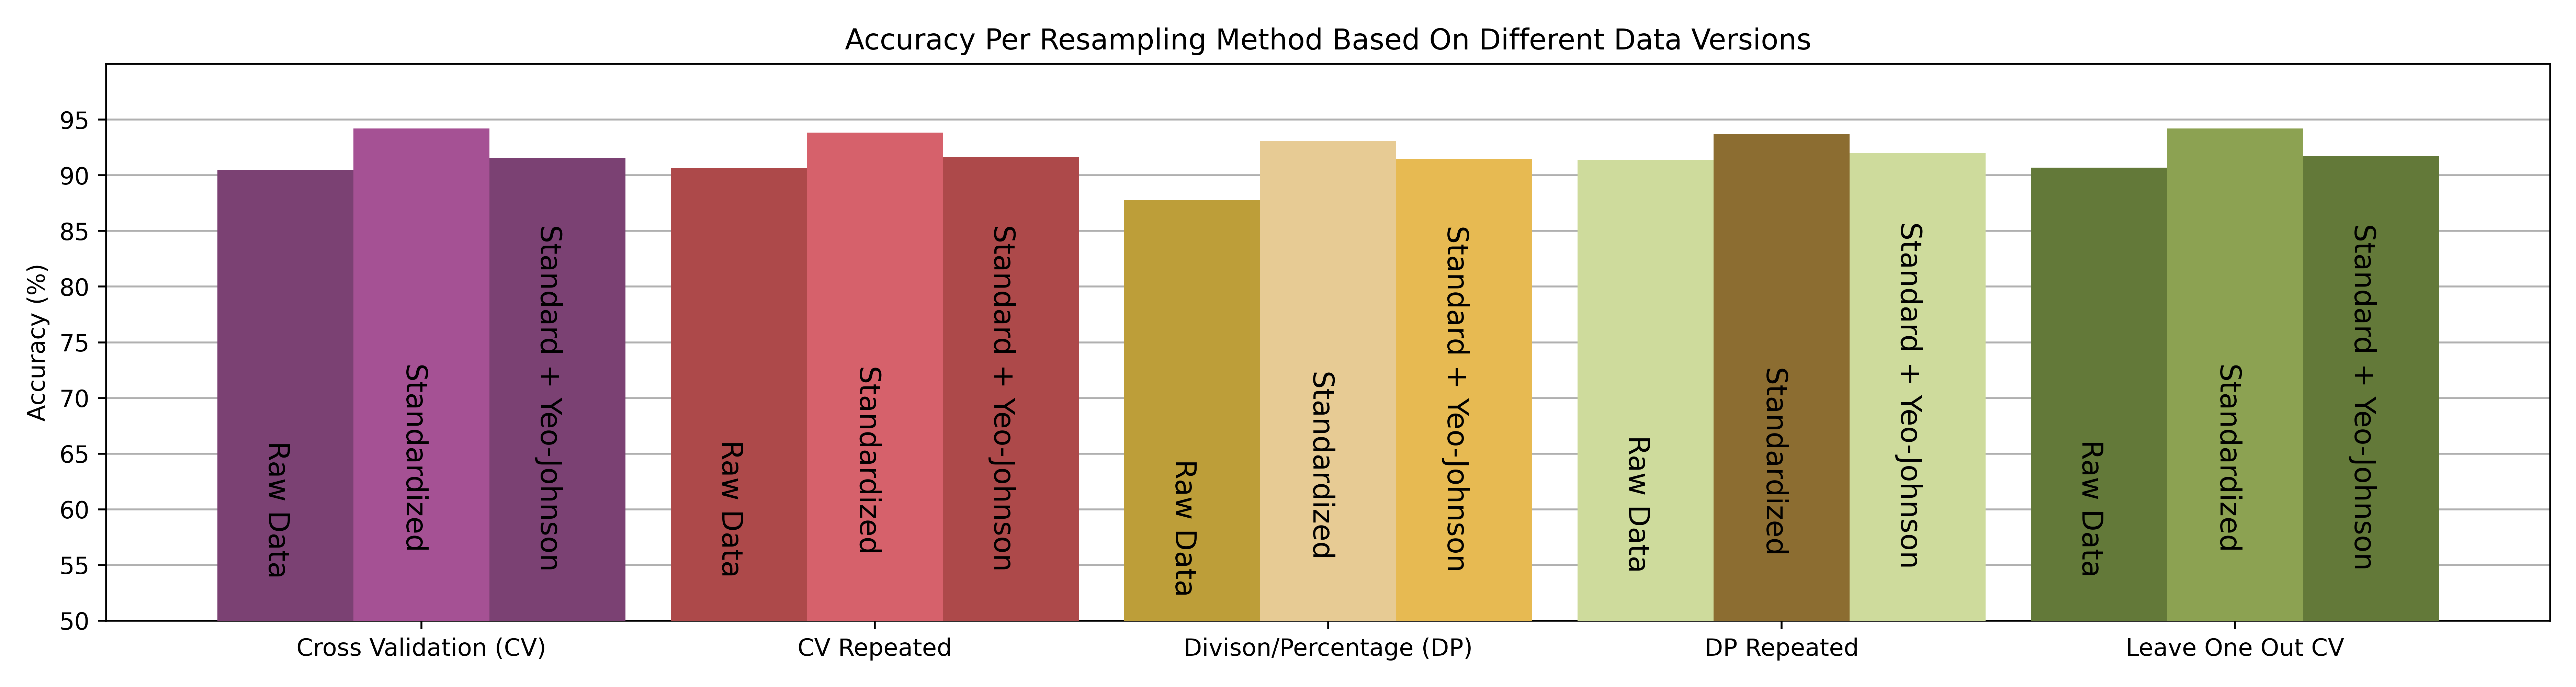
\includegraphics[width=7in]{acc-plot2.png}
    \caption{Prediction accuracy mean results by validation method}
    \label{fig:bars}
\end{figure}

Now we can easily conclude that, throughout every validation method, the lowest accuracy was reached when using raw data, followed by when the method used Standardized and Yeo-Johnson transformed data, and the highest accuracy was reached when using only Standardized data. The fastest but lowest accuracy can be reached with Division by Percentage method, while the slowest method was Leave One Out Cross Validation, due to the iterations depending on the amount of columns of the data set.
\\

Nevertheless, the accuracy in prediction using all these methods is quite high in general, surrounding the values of 87\%-94\%. This might look as too high even, and most probably will appear as an over-trained model when new input data is provided outside of the provided database and the accuracy decreases. I could be mistaken however, and the new input data set might as well result in similar accuracy levels, meaning that the model was not over-trained but actually extremely precise, which could be the case since Kaggle's data sets are very curated and maintained.
\\

However, one thing that indeed surprises is the accuracy level with a Standard and Yeo-Johnson transformation: the purely Standardized data set decreases the computation time in all methods compared to the method applied with raw data, but with a Standard and Yeo-Johnson transformation the accuracy is increased compared to raw data but decreased compared to only Standardized data. This is surprising because, in theory, Machine Learning algorithms such as Logistic Regression actually expect data centered in $\mu = 0$ and $\sigma = 1$ (Standardized) and that resembles a Gaussian Bell distribution, which is exactly what Yeo-Johnson's method does to data. But why is the accuracy not the highest with this two transforms that deliver data as expected by Logistic Regression? Let's look at Figure \ref{fig:lambdas}.

\begin{figure}[!ht]
\centering
    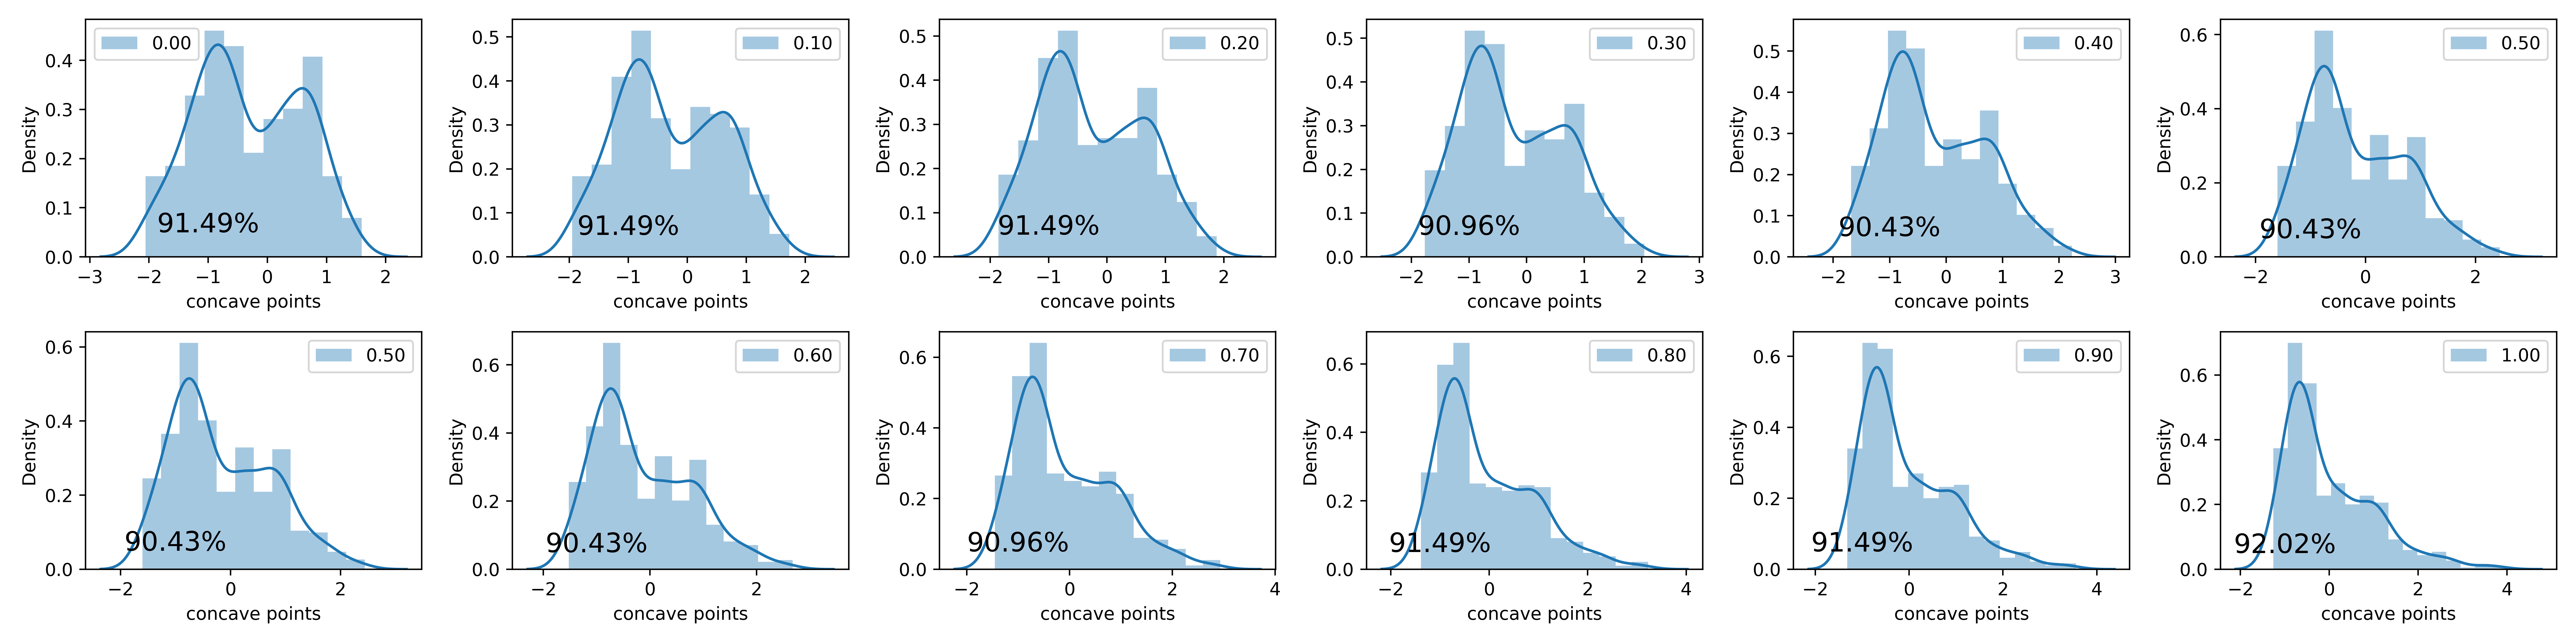
\includegraphics[width=7in]{lambdas.png}
    \caption{Lambda custom setting for Yeo-Johnson Transformation applied to one column.}
    \label{fig:lambdas}
\end{figure}

The answer to this might rely on the \textit{lambda} values that Yeo-Johnson's method fits to each column. By looking at Figure \ref{fig:lambdas}, where a sample column, in this case \verb$concave points$, is taken to suffer a custom lambda setting each time in order to cover the full range from -1 to 1 and then calculate the new accuracy of the model with this transform, we can see that there is one value of this lambda that increase the accuracy percentage (percentage shown in the lower left corner of each plot in Figure \ref{fig:lambdas}) of the \textbf{overall} set of data columns, which is exactly a lambda of 1.00, which represent a no transform value that leaves the column with the same distribution shape as in Figure \ref{fig:stand}. If we set this column to a transformation with a lambda of 1.0, we increase the overall accuracy to 92.02\%, whereas the fitted lambda value of the method (0.11) shows an overall accuracy of 91.49\%. Thus, the conclusion might be that Yeo-Johnson method can increase the accuracy of the model, but some manual changes to the calculated lambdas are needed.
\\

To finish, the conclusion for this data set specifically would be that the fastest method is Division by Percentage, with the data version being the Standardized data set, so that the model can converge in a much lesser amount of iterations. But Cross Validation seems to do a better job at the controlled but still random sets of data, producing the highest accuracy with Standardized data.

\printbibliography
% ////////////////////////////////////////////////////////////
%     Info ends
% ////////////////////////////////////////////////////////////
 
\end{document}
